\documentclass[journal,12pt,twocolumn]{IEEEtran}
\IEEEoverridecommandlockouts
\usepackage{cite}
\usepackage{amsmath,amssymb,amsfonts,bm}
\usepackage{mathtools}
\usepackage{tkz-euclide} 
\usetikzlibrary{calc,math}
 \usepackage{caption}
\usepackage{listings}
\usetkzobj{all}
\let\vec\mathbf
\newcommand{\myvec}[1]{\ensuremath{\begin{pmatrix}#1\end{pmatrix}}}
\newcommand{\norm}[1]{\left\lVert#1\right\rVert}


\begin{document}

\title{Assignment 3}

\author{\IEEEauthorblockN{Pulkit Saxena}}
\maketitle
\section{Question 1.36 Geolin.pdf }
BE and CF are two equal altitudes of a triangle ABC. Using RHS congruence rule, prove that the triangle ABC is isosceles.
\section{Solution}

BE and CF are two equal altitudes of a triangle ABC.
\captionsetup{justification=centering}

\begin{figure}[!h]
\centering
\resizebox{.5\columnwidth}{!}
{
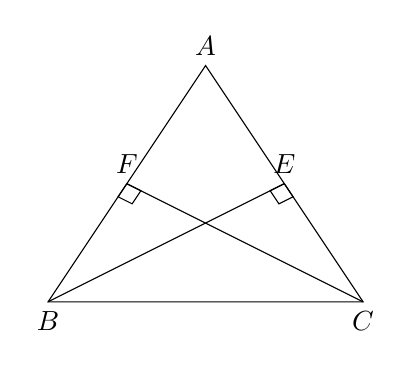
\begin{tikzpicture} 
        \coordinate (A) at (2, 3) {};
        \coordinate (B) at (0, 0) {};
        \coordinate (C) at (4, 0) {};
        \coordinate (F) at (1, 1.5) {};
        \coordinate (E) at (3, 1.5) {};
\draw (A)node[above]{$A$}--(B)node[below]{$B$}--(C)node[below]{$C$}--cycle;
\draw (B)node[below]{}--(E)node[above]{$E$};
\draw (C)node[below]{}--(F)node[above]{$F$};
\tkzMarkRightAngle[size=.2](B,E,C);
\tkzLabelAngle[dist=.5](B,E,C){};
\tkzMarkRightAngle[size=.2](C,F,B);
\tkzLabelAngle[dist=.5](C,F,B){};
\end{tikzpicture}
}
\caption{Triangle with equal altitudes on two sides}
\label{myfig}
\end{figure}
Given:-\\
1) Altitudes are Equal means their magnitude are same
 \begin{align}
 	\norm{\vec{E} - \vec{B}} = \norm{\vec{F} - \vec{C}} \label{1}
 \end{align}
2) Altitude makes right angle at the base therefore $\cos 90 =0$ therefore  FC $\perp$ BF and EB $\perp$ CE where $\textbf{m}$ is the directional vectors.
\begin{align}
\textbf{m}_{FC} \textbf{m}_{BF} = 0 \label{2}\\
\textbf{m}_{EB} \textbf{m}_{CE} = 0 \label{3}
\end{align}

From \eqref{2}
\begin{align}
    \left(\vec{B}-\vec{F}\right)\left(\vec{F}-\vec{C}\right)^T=\vec{0} && \left(\vec{F}-\vec{C}\right)\left(\vec{B}-\vec{F}\right)^T=\vec{0}\label{4}
\end{align}
From \eqref{2} and using \eqref{4} 
\begin{align}
    \left(\vec{B}-\vec{C}\right)\left(\vec{B}-\vec{C}\right)^T\\
    =\left(\vec{B}-\vec{F}+\vec{F}-\vec{C}\right)\left(\vec{B}-\vec{F}+\vec{F}-\vec{C}\right)^T)
    \end{align}
    \begin{align}
      =\left(\vec{B}-\vec{F}\right)\left(\vec{B}-\vec{F}\right)^T+\left(\vec{F}-\vec{C}\right)\left(\vec{F}-\vec{C}\right)^T 
    \end{align}
\begin{align}
   \norm{\vec{B}-\vec{C}}^2=\norm{\vec{B}-\vec{F}}^2+\norm{\vec{F}-\vec{C}}^2\label{8} 
    \end{align}
    Similarly\\
    From \eqref{3}
    \begin{align}
        \left(\vec{E}-\vec{B}\right)\left(\vec{E}-\vec{C}\right)^T=0 && \left(\vec{E}-\vec{C}\right)\left(\vec{B}-\vec{E}\right)^T=\vec{0}\label{9}
        \end{align}
From  \eqref{3} and using \eqref{9}  
\begin{align}
    \left(\vec{B}-\vec{C}\right)\left(\vec{B}-\vec{C}\right)^T\\
    =\left(\vec{B}-\vec{E}+\vec{E}-\vec{C}\right)\left(\vec{B}-\vec{E}+\vec{E}-\vec{C}\right)^T
    \end{align}
    \begin{align}
      =\left(\vec{B}-\vec{E}\right)\left(\vec{B}-\vec{E}\right)^T+\left(\vec{E}-\vec{C}\right)\left(\vec{E}-\vec{C}\right)^T 
    \end{align}
\begin{align}
   \norm{\vec{B}-\vec{C}}^2=\norm{\vec{B}-\vec{E}}^2+\norm{\vec{E}-\vec{C}}^2\label{13}
    \end{align}        
    Equating \eqref{8} and \eqref{13} and using \eqref{1}
    \begin{align}
      \norm{\vec{B}-\vec{F}}^2+\norm{\vec{F}-\vec{C}}^2 = \norm{\vec{B}-\vec{E}}^2+\norm{\vec{E}-\vec{C}}^2  
    \end{align}
    \begin{align}
       \norm{\vec{B}-\vec{F}}^2=\norm{\vec{E}-\vec{C}}^2\\
       =\norm{\vec{B}-\vec{F}}=\norm{\vec{E}-\vec{C}}\label{16}
    \end{align}
    
    Let $\angle FBC=\theta_1$  and  $\angle EBC=\theta_2$
    \begin{align}
        \left(\vec{B}-\vec{F}\right)\left(\vec{B}-\vec{C}\right)^T=\norm{\vec{B}-\vec{F}}\norm{\vec{B}-\vec{C}}\cos\theta_1\\
        \cos{\theta_1}=\frac{\left(\vec{B}-\vec{F}\right)\left(\vec{B}-\vec{C}\right)^T}{\norm{\vec{B}-\vec{F}}\norm{\vec{B}-\vec{C}}}\\
        \cos{\theta_1}=\frac{\left(\vec{B}-\vec{F}\right)\left(\vec{B}-\vec{F}+\vec{F}-\vec{C}\right)^T}{\norm{\vec{B}-\vec{F}}\norm{\vec{B}-\vec{C}}}\\
        \cos{\theta_1}=\frac{\left(\vec{B}-\vec{F}\right)\left(\vec{B}-\vec{F}\right)^T +\left(\vec{B}-\vec{F}\right)\left(\vec{F}-\vec{C}\right)^T}{\norm{\vec{B}-\vec{F}}\norm{\vec{B}-\vec{C}}}
        \end{align}
        From \eqref{4}
        \begin{align}
          \cos{\theta_1}=\frac{\left(\vec{B}-\vec{F}\right)\left(\vec{B}-\vec{F}\right)^T}{\norm{\vec{B}-\vec{F}}\norm{\vec{B}-\vec{C}}} \\
          \cos{\theta_1}=\frac{\norm{\vec{B}-\vec{F}}^2}{\norm{\vec{B}-\vec{F}}\norm{\vec{B}-\vec{C}}}\\
          \cos{\theta_1}=\frac{\norm{\vec{B}-\vec{F}}}{\norm{\vec{B}-\vec{C}}}
        \end{align}
        Similarly for $\angle EBC=\theta_2$
       \begin{align}
        \left(\vec{C}-\vec{E}\right)\left(\vec{B}-\vec{C}\right)^T=\norm{\vec{C}-\vec{E}}\norm{\vec{B}-\vec{C}}\cos\theta_2\\
        \cos{\theta_2}=\frac{\left(\vec{C}-\vec{E}\right)\left(\vec{B}-\vec{C}\right)^T}{\norm{\vec{C}-\vec{E}}\norm{\vec{B}-\vec{C}}}\\
        \cos{\theta_2}=\frac{\left(\vec{C}-\vec{E}\right)\left(\vec{B}-\vec{E}+\vec{E}-\vec{C}\right)^T}{\norm{\vec{C}-\vec{E}}\norm{\vec{B}-\vec{C}}}\\
        \cos{\theta_2}=\frac{\left(\vec{C}-\vec{E}\right)\left(\vec{B}-\vec{E}\right)^T +\left(\vec{C}-\vec{E}\right)\left(\vec{E}-\vec{C}\right)^T}{\norm{\vec{C}-\vec{E}}\norm{\vec{B}-\vec{C}}}
        \end{align}
        From {\eqref{9}}
        \begin{align}
          \cos{\theta_2}=\frac{\left(\vec{C}-\vec{E}\right)\left(\vec{C}-\vec{E}\right)^T}{\norm{\vec{C}-\vec{E}}\norm{\vec{B}-\vec{C}}} \\
          \cos{\theta_2}=\frac{\norm{\vec{C}-\vec{E}}^2}{\norm{\vec{C}-\vec{E}}\norm{\vec{B}-\vec{C}}}\\
          \cos{\theta_2}=\frac{\norm{\vec{C}-\vec{E}}}{\norm{\vec{B}-\vec{C}}}
        \end{align}
        From \eqref{16} we know $\norm{\vec{B}-\vec{F}}=\norm{\vec{E}-\vec{C}}$ we conclude
        \begin{align}
            \cos\theta_1=\cos\theta_2
            \implies\theta_1=\theta_2
        \end{align}
        So the sides opposite to equal angles are equal. Hence AB=AC hence the given Triangle is isosceles.
    \end{document}


